\documentclass[tikz]{standalone}
%\usepackage[showframe]{geometry}
%\geometry{
%paperwidth=6in,
%paperheight=8in
%}
\usepackage{siunitx}
\usetikzlibrary{shapes.callouts,arrows,calc}
\tikzset{
    level/.style = {
    	ultra thick,
    	black,
    },
    levelcentre/.style = {
    	dashed,
    	black
    },
    connect/.style = {
    	dashed,
    	black%red
    },
    label/.style = {
    	text width=2cm
    },
    frequency/.style = {
    	>=latex,
    	<->
    }
}
\begin{document}
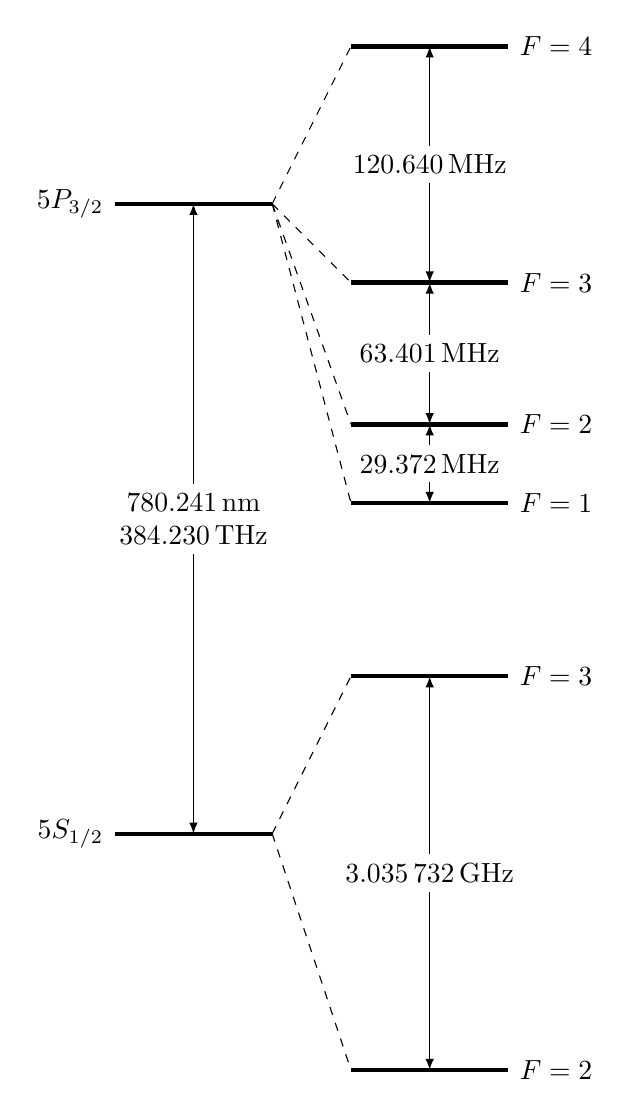
\begin{tikzpicture}[every node/.append style={fill=white}]

	% Coordenadas importantes
	\coordinate (S) at (0,0);
	\coordinate (P) at (0,8);
	\coordinate (end) at (2,0);
	\coordinate (mid) at (1,0);
	
	\path (S) + (3,0) coordinate (SC);
	\path (P) + (3,0) coordinate (PC);
	
	\path (S) + (3,-3) coordinate (SF2);
	\path (S) + (3,2) coordinate (SF3);
	
	\path (P) + (3,-3.8) coordinate (PF1);
	\path (P) + (3,-2.8) coordinate (PF2);
	\path (P) + (3,-1) coordinate (PF3);
	\path (P) + (3,2) coordinate (PF4);
	
    % Draw all levels
	\draw[level] (S) node[left] {$5S_{1/2}$} (S) -- ($(S)+(end)$);
	\draw[level] (P) node[left] {$5P_{3/2}$} (P) -- ($(P)+(end)$);
	
%	\draw[levelcentre] (SC) -- ($(SC)+(end)$);
%	\draw[levelcentre] (PC) -- ($(PC)+(end)$);
	
	\draw[connect] 
	($(S)+(end)$) -- (SF2) 
	($(S)+(end)$) -- (SF3);
	
	\draw[level] (SF2) -- ($(SF2)+(end)$) node[right] {$F=2$};
	\draw[level] (SF3) -- ($(SF3)+(end)$) node[right] {$F=3$};

	\draw[connect] 
	($(P)+(end)$) -- (PF1) 
	($(P)+(end)$) -- (PF2) 
	($(P)+(end)$) -- (PF3)
	($(P)+(end)$) -- (PF4);
	
	\draw[level] (PF1) -- ($(PF1)+(end)$) node[right] {$F=1$};
	\draw[level] (PF2) -- ($(PF2)+(end)$) node[right] {$F=2$};
	\draw[level] (PF3) -- ($(PF3)+(end)$) node[right] {$F=3$};
	\draw[level] (PF4) -- ($(PF4)+(end)$) node[right] {$F=4$};
	
	% Separaciones de niveles
	\draw[frequency] ($(S)+(mid)$) -- node[midway, text width=3cm, align=center] {\SI{780.241}{\nm} \SI{384.230}{\THz}} ($(P)+(mid)$);
	
%	\draw[frequency] ($(SC)+(mid)$) -- node[midway] {\SI{1.770}{\GHz}}($(SF2)+(mid)$);
	\draw[frequency] ($(SF2)+(mid)$) -- node[midway] {\SI{3.035732}{\GHz}}($(SF3)+(mid)$);
	
	\draw[frequency] ($(PF2)+(mid)$) -- node[midway] {\SI{29.372}{\MHz}}($(PF1)+(mid)$);
	\draw[frequency] ($(PF3)+(mid)$) -- node[midway] {\SI{63.401}{\MHz}}($(PF2)+(mid)$);
%	\draw[frequency] ($(PC)+.6*(mid)$) -- node[midway,right] {\SI{20.435}{\MHz}}($(PF3)+.6*(mid)$);
	\draw[frequency] ($(PF3)+(mid)$) -- node[midway] {\SI{120.640}{\MHz}}($(PF4)+(mid)$);

\end{tikzpicture}
\end{document}